\documentclass[10pt,a4paper]{article}
\usepackage[utf8]{inputenc} % para poder usar tildes en archivos UTF-8
\usepackage[spanish]{babel} % para que comandos como \today den el resultado en castellano
\usepackage{a4wide} % márgenes un poco más anchos que lo usual
\usepackage[conEntregas]{caratula}
\usepackage{mathtools}
\usepackage{float}
\usepackage[pdftex]{graphicx}
\usepackage{caption}
\usepackage{subcaption}
%\usepackage{Sty/algorithm2e}
\usepackage[ruled,vlined]{algorithm2e}
%Esto de abajo es para encabezado y pie de pagina
\usepackage{lastpage}
\usepackage{fancyhdr}
\usepackage{amsfonts}
\usepackage{verbatim}
\usepackage{wrapfig}
\usepackage{multirow}
\usepackage{ulem} 

\pagestyle{fancy}
%\fancyhf{} % clear all header and footer fields
%\fancyfoot[R]{\footnotesize Página \thepage\ de \lastpage\}

\cfoot{\thepage /\pageref{LastPage} }

\begin{document}

\titulo{Trabajo Práctico \#2}
\subtitulo{Histórico de Competiciones}

\fecha{\today}

\materia{Bases de Datos}
\grupo{Grupo 7}

% Pongan cuantos integrantes quieran
\integrante{Abdala Leila}{950/12}{abdalaleila@gmail.com}
\integrante{Bernaus Andres}{699/10}{andres.bernaus@hotmail.com}
\integrante{Gonzalez Alejandro}{32/13}{gonzalezalejandro1592@gmail.com}
\integrante{Romero Lucas}{440/12}{lucasrafael.romero@gmail.com}

\maketitle

\newpage
\tableofcontents

\newpage
\section{Introducci\'on}

Para esta segunda parte del trabajo practico, se desea modelar e implementar el historial de las competiciones mundiales; incluyendo el histórico de árbitros y escuelas que participaron en cada campeonato, los enfrentamientos por categoría y sus respectivos medalleros. 

El objetivo principal de esta base de datos ser\'a, en primer lugar, responder a las consultas requeridas en el enunciado. Por lo tanto, nos concentraremos fuertemente en modelar los documentos de la misma, para así poder resolverlas eficientemente.

\section{Modelo}

A continuación veremos en detalle los distintos aspectos del problema a
 resolver, y como decidimos modelarlos para cumplir con los 
 requerimientos del problema. \\ \\
 
Se nos pide, en primer lugar, guardar para cada campeonato y cada 
categoria de dicho campeonato, todos los enfrentamientos con sus 
resultados y medallas. Podemos modelar esto de la siguiente manera:\\ \\

\begin{itemize}

\item En primer lugar tenemos una relacion $N,M$, entre los campeonatos y 
los arbitros que participaron en dicho campeonato. De la misma manera, 
existe una relación $N,M$ entre los competidores y un campeonato determinado, 
y las escuelas y un campeonato.\\

\item El campeonato debe estar relacionado con la entidad enfrentamientos.
Como cada enfrentamiento esta directamente asociado a una categoria y a 
un campeonato, entonces podemos modelar una relacion 1 a 1 entre enfrentamiento
y su modalidad; y una relacion 1 a N entre el campeonato y sus enfrentamientos.\\

\item Por último, los campeonatos deben conocer los medalleros correspondientes a 
cada categoria. Luego necesariamente debemos modelarlo como una relacion 
$N,M$ entre el medallero y el campeonato.\\

\end{itemize}

Además de cumplir con los requerimientos básicos del enunciado, debemos asegurarnos 
de modelar el problema de tal manera que las consultas puedan resolverse 
eficientemente. \\

Algunas relaciones triviales que se desprenden de las consultas son: 
los enfrentamientos estan relacionados con competidores; las escuelas están 
relacionadas con competidores. \\ \\

Luego el Diagrama de entidad relacion para este problema es:


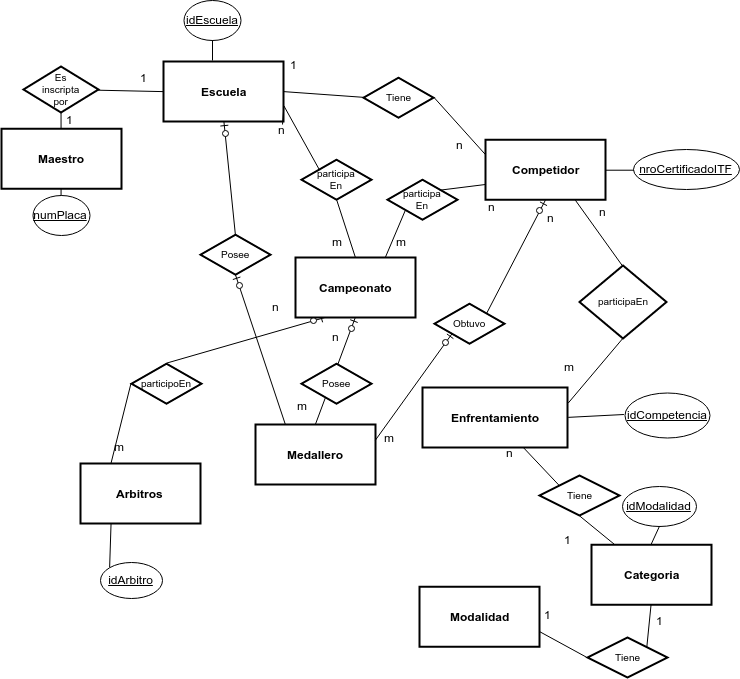
\includegraphics[scale=0.55]{diagDer.png}
 
 Un aspecto a tener en cuenta es que a diferencia del TP1, como tenemos 
 datos historicos. los datos de peso graduacion y edad no se van a corresponder
 con las restricciones  de cada compentencia. Es decir, podria llegar a tener a 
 un competido de 40 años, pero en su historial figura que compitio en una categoria
 de hasta 30 años. Lo Cual tiene sentido si dicha competencia ocurrior con 
 bastante más anterioridad.\\


\newpage
\section{Diagrama de Interrelación de Documentos}

Una vez obtenido el diseño de la base de datos que deseamos modelar, 
el siguiente paso es comenzar a transformar dicho modelo en un esquema 
de documentos. Para ello utilizamos el Diagrama de interelacion de 
Documentos, con el objetivo de poder ilustrar como nuestro modelo 
resuelve las consultas del enunciado de forma eficiente. Para ello
iremos viendo cada consulta y trateremos de modelar los documentos 
en base a ellos.\\ \\

\subsection{Consultas}

La \textbf{primera consulta} requiere: devolver la cantidad de enfrentamientos ganados 
por competidor para un campeonato dado. Es decir, que si busco un registro 
particular de Campeonato, necesitamos poder devolver tuplas de 
$(competidor,cantidadDeEnfrentamientosGanados)$. En consecuencia, además de
contar con la lista de competidores que participaron en cada Campeonato, 
almacenaremos tambien sus cantidades de enfrentamientos ganados.\\

Para la \textbf{segunda consulta} y \textbf{tercera consulta}, se necesita poder obtener las 
cantidades de medallas pr campeonato y el total de medallas en la historia
(consultas 2.3 y 2.2 respectivamente). Usando el mismo razonamiento que en 
la consulta anterior; almacenamos un arreglo de campeonatos junto a la cantidad 
de medallas obtenidas en el mismo. Luego resolver la consulta se reduce a sumar 
todas las medallas, en el caso de la 2.2, y encontrar el maximo valor para la 
consulta 2.3. \\

El caso del punto \textbf{2.4} quedo resuelto en la etapa de diseño. Como los arbitros 
poseen una lista con sus participaciones en los campoeonatos, podemos resolver 
esta consulta fácilmente tomando el tamaño de la misma. \\ 

Para la \textbf{consulta 2.5} volvemos a interactuar con campeonatos y competidores
de forma similar a la primer consulta. La única diferencia es que ahora 
necesitamos conocer las escuelas a las cuales pertenecen los competidores.
La solución que encontramos fue la siguiente: reorganizar la lista de competidores de 
cada y agruparlos por Escuela. De esta manera, podemos contabilizar rápidamente la
cantidad de competidores por Escuela, y ademas cumplir con las consultas 2.2 y 2.3.\\

Para la \textbf{ultima consulta (2.6)} se nos pide obtener los competidores que más 
medallas obtuvieron por categoria. Para ello decidimos incluir en el $Competidor$, un 
campo por cada una de las categorias en el cual se lleve la cuenta de las 
medallas obtenidas por dicho competidor. Luego, para resolver la consulta, 
podemos recorrer la tabla de competidores y quedarnos con aquellos  que 
tengan mayor cantidad de medallas en alguna de las categorias. \\ ||

Teniendo en cuenta estas consideraciones, el diagrama de interrelación de 
Documentos resultante será:\\ \\

%\includegraphics[scale=0.75]{did.png}



 




\newpage
\section{Json Schema}

  \begin{verbatim}
    "Campeonato":{
    "properties": {
        "Medallero": {
            "items": {
                "properties": {
                    "idCategoria": {
                        "type": "integer"
                    },
                    "idPrimerCompetidor": {
                        "type": "integer"
                    },
                    "idSegundoCompetidor": {
                        "type": "integer"
                    },
                    "idTercerCompetidor": {
                        "type": "integer"
                    }
                },
                "type": "object"
            },
            "type": "array"
        },
        "arbitros": {
        	"items":{
        		"properties": {
        			"idArbitro":{
        				"type": "integer"
        			}
        		}
        	},
            "type": "array"
        },
        "año": {
            "type": "integer"
        },
        "escuelas": {
            "items": {
                "properties": {
                "datos": {
                    "items": {
                        "properties": {
                            "cantEnfrentamientos": {
                                "type": "integer"
                            },
                            "nombreCompetidor": {
                                "type": "string"
                            }
                        },
                        "type": "object"
                    },
                    "type": "array"
                },
                "nombreEscuela": {
                    "type": "string"
                }
            },
                "type": "object"
            },
            "type": "array"
        },
        "required":["año","escuelas","arbitros"]
    },
    "type": "object"
}
\end{verbatim}
  \begin{verbatim}


"Categoria":{
    "properties": {
        "Edad": {
            "properties": {
                "max": {
                    "type": "integer"
                },
                "min": {
                    "type": "integer"
                }
            },
            "type": "object"
        },
        "Graduacion": {
            "type": "integer"
        },
        "Modalidad": {
            "type": "string"
        },
        "Peso": {
            "properties": {
                "max": {
                    "type": "integer"
                },
                "min": {
                    "type": "integer"
                }
            },
            "type": "object"
        },
        "idCategoria": {
            "type": "integer"
        },
        "required":["Edad","Graduacion","Modalidad","Peso","idCategoria"]
    },
    "type": "object"
}
  \end{verbatim}
  \begin{verbatim}

"Enfrentamiento": {
    "properties": {
        "Competidores": {
            "items": {
                "type": "integer"
            },
            "type": "array"
        },
        "Ganador": {
            "type": "integer"
        },
        "idCategoria": {
            "type": "integer"
        },
        "idEnfrentamiento": {
            "type": "integer"
        },
        "required":["Competidores","Ganador","idCategoria","idEnfrentamiento"]
    },
    "type": "object"
}
  \end{verbatim}
  \begin{verbatim}  
"escuela":{
	"type":"object",
	"properties":{
		"nombreMaestro":{"type":"string"},
		"apellidoMaestro":{"type":"string"},
		"graduacionMaestro":{"type":"number", "multipleOf": 1.0,"minimum":1,"maximum":6},
		"nroPlacaInstructor":{"type":"string"},
		"pais":{"type":"string"},
		"medallasPorCampeonato":{
			"type":"object"
			"properties":{
				"campeonato":{"type":"integer"},
				"cantMedallas":{"type":"number", "multipleOf": 1.0,"minimum":0},
			}
		},
		"required":["nombreMaestro","apellidoMaestro","graduacion","nroPlacaInstructor","pais"]
	}
}
  \end{verbatim}
  \begin{verbatim}
"arbitro":{
	"type":"object",
	"properties":{
		"nombre":{"type":"string"},
		"apellido":{"type":"string"},
		"graduacion":{"type":"number", "multipleOf": 1.0,"minimum":1,"maximum":6},
		"nroPlaca":{"type":"string"},
		"pais":{"type":"string"},
		"participoEn":{
			"type":"array",
			"items": {"type":"integer","uniqueItems":true}
		},
		"required":["nombre","apellido","graduacion","nroPlaca","pais"]
	}
}

  \end{verbatim}
  \begin{verbatim}
"competidor":{
	"type": "object",
	"properties": {
		"nombre": {
			"type": "string"
		},
		"apellido": {
			"type": "string"
		},
		"dni": {
			"type": "string"
		},
		"fechaNacimiento": {
			"type": "string",
			"format": "date-time"
		},
		"genero": {
			"type": "string",
			"enum": ["masculino", "femenino"]
		},
		"graduacion": {
			"type": "number",
			"multipleOf": 1.0,
			"minimum": 1,
			"maximum": 6
		},
		"nroCertificadoITF": {
			"type": "string"
		},
		"peso": {
			"type": "number",
			"multipleOf": 1.0,
			"minimum": 1
		},
		"nombreEscuela": {
			"type": "string"
		},
		"pais": {
			"type": "string"
		},
		"numMedallasCombate": {
			"type": "integer"
		},
		"numMedallasSalto": {
			"type": "integer"
		},
		"numMedallasRotura": {
			"type": "integer"
		},
		"numMedallasFormas": {
			"type": "integer"
		},
		"numMedallasEquipos": {
			"type": "integer"
		},
		"required": ["nombre", "apellido", "graduacion", "dni", "nombreEscuela", "nroCertificadoITF"]
	}
}

  \end{verbatim}

\section{Implementación  de Funcionalidades}

Una vez que terminado el modelo del problema, el siguiente paso fue comenzar a implementar la base de datos. Es decir generar en RethinkDB las distintas tablas, documentos y consultas necesarias para resolver el problema.\\

Para ello creamos un pequeño programa que genere de manera aleatoria todos los datos necesarios, asegurándose de ser consistente al momento de crear documentos para los enfrentamientos, campeonatos, escuelas y demás. Ya que, por ejemplo, si un competidor gana un enfrentamiento, el mismo debe ser contabilizado en el Documento $Campeonato$.\\ \\

Una vez llenadas las tablas con los suficientes datos, implementamos cada una de las consultas:\\ \\

\begin{itemize}

\item{\textbf{Cantidad de enfrentamientos ganados por competidor para un campeonato dado.}

Como esta consulta debe realizarse para un Campeonato determinado, el primer paso es filtrar la tabla $Campeonatos$ hasta obtener el documento indicado. Para ello utilizamos la función $filter$ sobre el campo $anio$ que, por lo visto anteriormente, identifica inequívocamente a cada Campeonato.\\

Una vez seleccionado el campeonato, hicimos un concatMap y un reduce sobre todos los pares $(competidor,enfrentamientosGanados)$ de todas las escuelas que participan del campeonato, obteniendo así los datos necesarios para esta consulta.

\begin{verbatim}

r.db('TP2').table('Campeonato').filter({anio: 2017})("escuelas")
.concatMap(function(elem){
  	return elem("competidores");
  })
  .reduce(function(left, right){
    return left.add(right);
  })

\end{verbatim}
}

\item{\textbf{Cantidad de medallas por nombre de escuela en toda la historia}

Usando la función map, podemos tomar cada documento $Escuela$ y devolver únicamente los campos que nos interesan para resolver la consulta, es decir, su $nombreEscuela$ y la sumatoria de todos los campos $cantidadMedallas$ que se encuentren en el arreglo $medallasPorCampeonato$.

\begin{verbatim}

r.db("TP2").table("Escuela").map(
function(elem){
  return {id: elem("idEscuela"),nombre: elem("nombreEscuela"),
    		cantidadTotal: elem("medallasPorCampeonato").sum("cantidadMedallas")};
	}
)

\end{verbatim}
}

\item{\textbf{Para cada escuela, el campeonato donde gan\' m\'as medallas}

De forma similar a la consulta anterior usamos una función $map$. La 
cual devolverá, $nombreEscuela$ junto con el an\~o del campeonato cuya tupla\\
 $(anio,cantidadMedallas)$ asociada sea máxima. Es decir, corresponda al 
 elemento de \\$medallasPorCampeonato$ con mayor cantidad de medallas.

\begin{verbatim}

r.db("TP2").table("Escuela").map(
  function(elem){
    var res = elem("medallasPorCampeonato").max("cantidadMedallas");
    return {escuela: elem("nombreEscuela"), campeonato: res("anio")};
  })

\end{verbatim}
}

\item{\textbf{Los arbitros que participaron en al menos 4 campeonatos}

Como cada documento $Arbitro$ contiene una lista con los an\~os de los campeonatos en los que participo, responder esta consulta significa filtrar aquellos árbitros que cumplan con la condición. Esto lo podemos hacer usando un $filter$ sobre el largo del arreglo $participoEn$, y devolviendo solo aquellos que tengan longitud mayor o igual a 4. 

\begin{verbatim}


r.db("TP2").table("Arbitro").filter(
function(elem){
  return elem("participoEn").count().ge(4);
})

\end{verbatim}
}

\item{\textbf{Las escuelas que han presentado el mayor numero de competidores en cada campeonato}

Usando un map podemos tomar cada campeonato, y como cada uno tiene asociado un arreglo con todas las escuelas, que a su vez contiene una lista con todos los competidores, podemos entonces responder a la consulta tomando el largo del arreglo de competidores, y comparándolo con las otras escuelas.

\begin{verbatim}


r.db('TP2').table('Campeonato').map(
  function(elem){

    var max = elem("escuelas").max(
      function(esc){
        return esc("competidores").count();
      })("competidores").count();
    
    return {anio: elem("anio"), escuelas: elem("escuelas").filter(
      function(val){
      	return val("competidores").count().eq(max)
      }).pluck("idEscuela","nombreEscuela")};
})

\end{verbatim}
}


\item{\textbf{Obtener los competidores que m\'as medallas obtuvieron por modalidad}

Para resolver esta consulta, calculamos primero la maxima cantiada de 
medallas por cada modalidad, y luego filtramos todos los competidores que 
cumplan con dicha cantidad de medallas


La consulta entonces quedaría:\\ \\

\begin{verbatim}

r.db('tp2').table("Competidor").filter(
  function(elem){
    var maximos = {
      formas: r.db('tp2').table("Competidor").max("formas")("formas"),
      salto: r.db('tp2').table("Competidor").max("salto")("salto"),
      rotura: r.db('tp2').table("Competidor").max("rotura")("rotura"),
      combate: r.db('tp2').table("Competidor").max("combate")("combate")
      };
    
    return elem("salto").eq(maximos["salto"]).or(
           elem("formas").eq(maximos["formas"]),
           elem("combate").eq(maximos["combate"]),
           elem("rotura").eq(maximos["rotura"]))
}).group(
  function(elem){
    var maximos = {
      formas: r.db('tp2').table("Competidor").max("formas")("formas"),
      salto: r.db('tp2').table("Competidor").max("salto")("salto"),
      rotura: r.db('tp2').table("Competidor").max("rotura")("rotura"),
      combate: r.db('tp2').table("Competidor").max("combate")("combate")
      };
    
    return elem("salto").eq(maximos["salto"]).branch(["salto"],[]).add(
           elem("formas").eq(maximos["formas"]).branch(["formas"],[])).add(
           elem("combate").eq(maximos["combate"]).branch(["combate"],[])).add(
           elem("rotura").eq(maximos["rotura"]).branch(["rotura"],[]))
    
  }, {multi: true})

\end{verbatim}
}

\item \textbf{El punto 2.8 queda resuelto en la consulta 2.3, la cual esta 
implementada con map reduce}

\end{itemize}

\subsection{Sharding}

Tomamos la tabla de Competidores, pues es la que tiene mayor cantidad de 
registros (alrededor de 2000), y creamos 3 shards. Inicialmente la base 
de datos particion\'o el total de los registros en un shard con 672 
registros, el segundo con 621 y el tercero con 561. Luego realizamos 
inserciones de a 100 competidores y obtuvimos los siguientes resultados: \\ \\

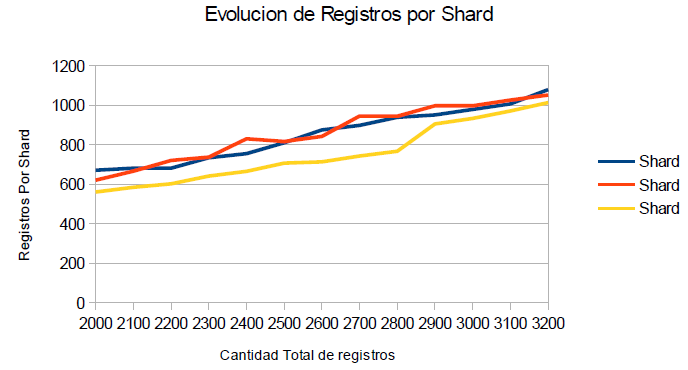
\includegraphics[scale=0.75]{Shards.png}

Como podemos ver en el grafico, rethinkDB distribuye equitativamente las 
inserciones a todos los shards, de manera de aliviar la carga de la base 
de datos al momento de responder consultas o realizar operaciones 
como inserciones.


\section{Conclusión}

Sobre este trabajo, queremos destacar algunas conclusiones a las que llegamos durante el transcurso del mismo. 


\end{document}
